\documentclass[conference]{IEEEtran}
%\IEEEoverridecommandlockouts
% The preceding line is only needed to identify funding in the first footnote. If that is unneeded, please comment it out.
\usepackage{cite}
\usepackage{amsmath,amssymb,amsfonts}
%\usepackage{algorithmic}
\usepackage{graphicx}
\usepackage{textcomp}
\usepackage{xcolor}
\def\BibTeX{{\rm B\kern-.05em{\sc i\kern-.025em b}\kern-.08em
    T\kern-.1667em\lower.7ex\hbox{E}\kern-.125emX}}

\usepackage{algorithm}
\usepackage{algpseudocode}
\usepackage{multirow}


\makeatletter
\def\BState{\State\hskip-\ALG@thistlm}
\makeatother

\newcommand\todo[1]{\textcolor{red}{TODO:}\textcolor{red}{#1}}

\begin{document}

\title{Project Proposal}

\author{\IEEEauthorblockN{Harshit Mahapatra}
\IEEEauthorblockA{\textit{Dept. of Computer Science} \\
\textit{Aarhus University}\\
Aarhus, Denmark \\
au608727@post.au.dk}
\and
\IEEEauthorblockN{Patrick Lewandowski}
\IEEEauthorblockA{\textit{Dept. of Computer Science} \\
\textit{Aarhus University}\\
Aarhus, Denmark \\
au614714@post.au.dk}
\and
\IEEEauthorblockN{Tomas Manuel Rebelo Mota}
\IEEEauthorblockA{\textit{Dept. of Computer Science} \\
\textit{Aarhus University}\\
Aarhus, Denmark \\
au614711@post.au.dk}
}

\maketitle

\section{Introduction}
We will fit the following sensors into a walker:
 -An accelerometer that will allow tracking of how much the walker is being used
 -A GPS that will allow the municipality to have an overview of the position of each user
 -Pulse sensors on each handle, in order to track the user's heart rate overtime	

These sensors will the be connected to an Arduino that transmits the data through LoRaWAN to a Raspberry PI that will be the LoRaWAN Gateway. 	

\section{Use case}
	All the people using the walker will be streaming their sensor data to a central server belonging to the Municipality. These data are then used to analyse both the overall use of the walkers, something that interests the manufacturing companies, and the over-time change of the health indicators in order to track long-term progress of the users well-being.

\section{Usage of Internet of Things}
	How: We will use sensors to gather data and send it to a remote server
	
Why: Seems like a good way to gather data from a moving object like a walker. Since the end goal is having all the data in a central server owned by the municipality and the infrastructure for LoRaWAN is already considerably developed in Aarhus, we thought that would be a good protocol to use. We considered the possibility of getting sensors with built-in LoRaWAN capabilities, but doing that would restrict our choice of sensors, they would be considerably more expensive, and the work to be done by us would be reduced, meaning a smaller "delta" in our project.
\section{Questions we seek to answer}
	Can we help make better walkers by analysing how and where they are used?
Is it possible to have a practical walker that measures some health parameters of its user? 
Can we track the health progress of a user by analysing the measured health parameters? We will probably not get to this point because our project intends to be the foundation for a larger scheme with the next steps including the analysis of collected data.

\section{The envisioned architecture}

\begin{figure}[H]
	\begin{center}
		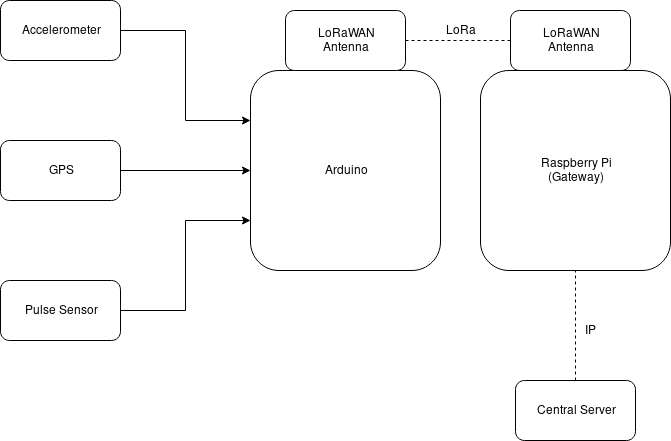
\includegraphics[width=0.3\textwidth]{images/Architecture.png}
		\caption[]{Schematic representation of the Architecture}
	\end{center}	
\end{figure}
\section{Weekly milestones}
	1- Have the Raspberry Pi(Gateway) communicating with server
2- Have Arduino communicating with Raspberry Pi using LoRaWAN
3- Connect Accelerometer to Arduino and get its data on Server
4- Repeat step 4 for GPS and pulse sensor
5- Fit Components on the walker and preliminary tests
6- Test system, collect and plot data
7- Write report


\bibliography{ref}
\bibliographystyle{ieeetr}

\end{document}
